\section{A first-principles model of the thrashing curve}\label{sec:fp}

Section~\ref{sec:fluid} takes $\mu(n)$ as measured. Here we \emph{predict} it, together with the all-miss level, the peak, the from-empty edge, the trapped state and the cap condition, from the pool size $M$, the workload of \S\ref{sec:notation}, the tool-time law, and the iteration-cost model of our simulator (\S\ref{sec:sim}), which was fitted only to server-log iteration timings. No parameter is fitted to any $\mu(n)$ point, from-empty outcome or trap measurement. Every proposition below is about a deterministic fluid model, and the layers of \S\ref{sec:fp-heur}, the trapped-state layer included, are heuristics; we do not prove that the engine converges to the model.

\begin{figure*}[t]\centering
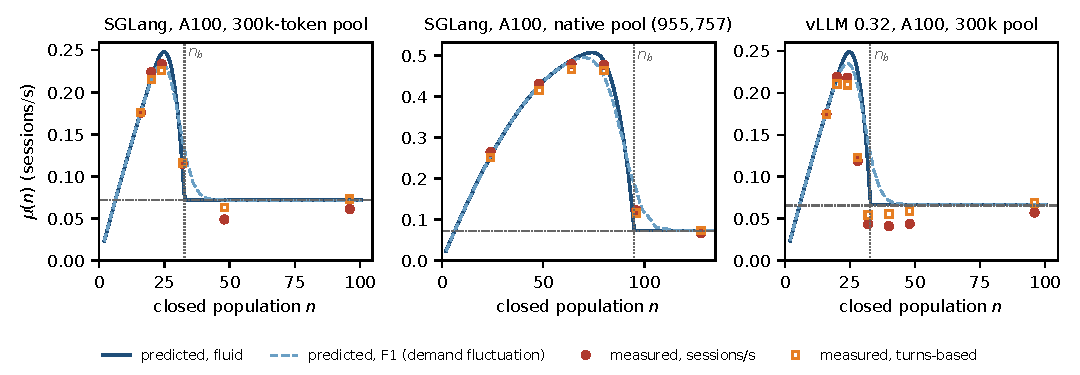
\includegraphics[width=\textwidth]{figs/fig8_theory_curves.pdf}
\caption{Predicted thrashing curves against the engine. Lines: the first-principles model (solid, fluid; dashed, with the demand-fluctuation layer F1). Its inputs are the pool, the workload and a cost model fitted to server-log timing only; vLLM and the H200 also get one speed factor fitted to their all-miss token rate. Points: measured $\mu(n)$, sessions/s (filled) and turns-based (open). Dotted: the predicted all-miss onset $n_b$ (Eq.~\eqref{eq:nb}); dash-dotted: the measured $\lref$. No measured $\mu(n)$ point enters any prediction. The first three panels are in sample: the model's authors knew every point. The fourth is out of sample: the H200 curve was predicted under tag \texttt{r13-theory-pred} before the model's authors read it; the runs at $n=36$, 44 and 52 (ringed) were submitted after the freeze and are blind in time, those at $n\le32$ (shaded) had been seen by the first author before it, and the others are blind by access only (\S\ref{sec:frozen}). The $n$ axis is logarithmic, as in Fig.~\ref{fig:curve}, and ends at 140, so the $n=300$ runs are not plotted. The measured points below $\lref$ beyond the cliff ($n=48$--96 at 300k, 128 with the native pool, 32--96 on vLLM) are not described by the stationary model; at 300k we attribute them to the synchronized start of the closed runs (\S\ref{sec:curve}).}\label{fig:fpmu}
\end{figure*}

\subsection{Model}\label{sec:fp-model}
Let $w_k=P(T\ge k)/E[T]$ be the turn mix, $E_k=L_k+d$ the KV of a session after turn $k$, $\bar E=\sum_k w_kE_k=10{,}569$ tokens, $A_1=\sum_k P(T\ge k+1)E_k=144{,}960$ the KV a session carries into tool calls over its life, $E[E_T]=11{,}045$ its final KV, $\bar z=E[Z]$, and $\bar z'=\bar z(1-1/E[T])$ its tool time per turn. The tool time $Z$ has distribution $F_Z$ and density $f$. \emph{Server.} At turn completion rate $\nu$ (turns/s) and follow-up hit probability $h$, turn $k$ needs prefill GPU time $t_k(h)=t^m_k-h\,\mathbf 1\{k\ge2\}(t^m_k-t^h_k)$, with $t^m_k,t^h_k$ the miss and hit prefill times of the cost model (a hit prefills $\Delta+1=551$ tokens). SGLang runs prefill and decode in separate iterations with prefill priority, so prefill takes a fraction $p=\nu\sum_kw_kt_k(h)$ of the GPU and the number $R_D$ of decoding requests solves $R_D(1-p)=\nu(d-1)\tau_D(R_D)$, where $\tau_D$ is the cost model's decode iteration time. A turn occupies the engine for $S_k=t_k(h)+S_D$ with $S_D=R_D/\nu$ and reserves its KV $E_k$ throughout, so running requests hold $K_{\mathrm{run}}(\nu,h)=\nu\sum_kw_kE_kS_k$ tokens. \emph{Memory.} Idle KV (sessions in tool calls, and the KV of finished sessions, which the engine cannot know is dead) is evicted least recently used first.
\begin{assumption}[Che~\citep{che2002hierarchical,fricker2012versatile}]
In stationarity an idle item is evicted at a deterministic idle age $R$.
\end{assumption}
\noindent By $H=\lambda G$ the idle KV is then $\mu\mathcal D(R)$ with $\mathcal D(R)=A_1E[\min(Z,R)]+E[E_T]R$, and the pool is full, so
\begin{equation}\label{eq:balance}
\begin{gathered}
M=K_{\mathrm{run}}(\nu,h)+\frac{\nu}{E[T]}\mathcal D(R),\qquad h=F_Z(R),\\
n=\nu\,(\bar S+\bar z'),\qquad \mu=\nu/E[T],
\end{gathered}
\end{equation}
the last two being Little's law with $\bar S=\sum_kw_kS_k$. Requests queue only when running reservations alone fill the pool ($K_{\mathrm{run}}=M$, hence $R=0$ and $h=0$). With $K_{\mathrm{run}}=0$ and no queue, Eq.~\eqref{eq:balance} is the characteristic-time equation of Yao et al.~\citep{yao2026multiturn} term for term. Three additions make the hit rate feed back on itself. Running reservations depend on $h$, because under prefill priority misses starve decode. Throughput is set by a server and a closed population, not by an exogenous arrival rate. And there is a memory-gated all-miss branch. On every partially hitting state the reuse gap is still the exogenous tool time; only on the all-miss branch does the queue set it.

\subsection{Results}\label{sec:fp-results}
\begin{proposition}[stationary states and the all-miss onset]\label{prop:nb}
Let $\nu_b$ solve $K_{\mathrm{run}}(\nu,0)=M$, $\mu_b=\nu_b/E[T]$, and $E_S=\sum_kw_kE_kS_k/\sum_kw_kS_k$ at $(\nu_b,0)$.
(a) Each $R>0$ gives exactly one queue-free stationary state; the states with a queue are exactly the all-miss states $(h=0,\nu=\nu_b)$; $\mu(n)=\mu_b$ for all large $n$, so $\mu_b$ is the model's $\lmiss$ and $\muinf$ (the model's counterpart of Proposition~\ref{prop:A} of Appendix~\ref{app:proofs}, with (A4)).
(b) All-miss states exist exactly for $n\ge n_b$, where
\begin{equation}\label{eq:nb}
n_b=\nu_b\,\bar z'+M/E_S,
\end{equation}
the sessions in tool calls at the all-miss rate plus one pool's worth of running sessions.
(c) If every GPU cost is divided by $s$ (a uniformly faster GPU), then $\nu_b\mapsto s\nu_b$, $E_S$ is unchanged, and $n_b(s)=n_b(1)+(s-1)\,\nu_b(1)\,\bar z'$.
\end{proposition}
\noindent At 300k, $n_b=4.94+27.76=32.70$ (native pool: 94.86; vLLM: 32.83). Parts (a) and (c), Proposition~\ref{prop:scaling}(b)--(c) and Proposition~\ref{prop:fold} rest on Lemmas~\ref{lem:server} and~\ref{lem:rho}, which are for the separate-iteration (SGLang) server; for vLLM's mixed iterations $n_b$ follows from the identity of part (b), which holds whenever the mixed server's $\nu_b$ exists, that is, while its chunk budget does not bind (Appendix~\ref{app:fp}). The pool part $M/E_S$ has the form of MISA-T's cap, a reserved block budget over a conservative session length~\citep{hong2026misat}, and of AgentKV's collapse predictor (from its abstract)~\citep{anon2026agentkv}. What is new is the tool-call term and the identification of $n_b$ as the onset of the all-miss branch. On the two SGLang cells the measured 0.5-hit crossing (32.2 and 93.4) lies just below $n_b$; on vLLM it lies at 29.1, nearer the pool part (28.2) than $n_b$. Part (c) says that a faster GPU moves the onset \emph{outward}: on an H200 at the same pool ($s=2.742$, fitted to its all-miss token rate) $n_b=41.3$. On the H200 the measured crossing moved out, from 32.2 to about 38.9, though past it the engine lost its hits more gradually than the model (\S\ref{sec:h200}, \S\ref{sec:frozen}).

\begin{proposition}[speed and tool time enter only through $s\bar z$]\label{prop:scaling}
Write $\omega=\mu^*/\mu_b$ for the peak ratio and $Z=\bar zY$ with $Y$ fixed. (a) $\lmiss(\mathcal C/s)=s\,\lmiss(\mathcal C)$ and $\omega(\mathcal C/s,\bar z)=\omega(\mathcal C,s\bar z)$ exactly, for cost model $\mathcal C$. (b) $\omega$ is non-increasing in $s\bar z$, strictly while $\omega>1$. (c) $\omega\to1$ as $s\bar z\to\infty$.
\end{proposition}
\noindent Faster GPUs therefore lower the peak ratio, the upper end of the window when the from-empty edge does not bind: the good state is limited by memory and tool time, neither of which speeds up. The same holds for slower tools. On the H200 the measured peak ratio against $\lref$ was 1.89 (turns-based), against 3.15 on the A100 and 1.92 predicted (\S\ref{sec:frozen}); this comparison is not blind to the first author, who had seen the H200 values for $n\le32$ before the freeze.

\begin{proposition}[exogenous gaps cannot produce the cliff]\label{prop:E}
Suppose that the reuse gap of every follow-up is its tool time $Z$, with no queue wait, that running requests hold $K\ge0$ tokens of the pool, and that idle KV is evicted at a deterministic idle age $R$ (Assumption MF), so that $M-K=\lambda_0\,\mathcal D(R)$ at session throughput $\lambda_0$. Then $R\ge(M-K)/(\lambda_0E[T]\bar E)$, so the follow-up hit probability $F_Z(R)$ is at least $F_Z\big((M-K)/(\lambda_0E[T]\bar E)\big)$; and if $F_Z$ is continuous and strictly increasing, a follow-up hit probability of at most $h$ requires $K\ge M-\lambda_0\,\mathcal D(F_Z^{-1}(h))$.
\end{proposition}
\begin{proof}
Since $\min(Z,R)\le R$ and $A_1+E[E_T]=\sum_kP(T\ge k)E_k=E[T]\bar E$, we have $\mathcal D(R)\le E[T]\bar E\,R$, which gives the first bound, $F_Z$ being non-decreasing. A hit probability of at most $h$ means $R\le F_Z^{-1}(h)$, and $\mathcal D$ is increasing.
\end{proof}
\noindent With $K=0$ the balance is the characteristic-time equation of Yao et al.~\citep{yao2026multiturn}, and the proposition says that a hit probability near zero needs running requests to hold almost the whole pool, which in our model happens only on the all-miss branch, where requests queue and the queue sets the gap (Proposition~\ref{prop:nb}(a)). Evaluated retrospectively at the measured throughput of each closed run, with nothing fitted, exogenous-gap closures decay smoothly in $n$ and never reach the measured zeros: at $n=48$ on the 300k pool, where no turn hit, Yao et al.'s fixed point gives a hit fraction of 0.93, the same equation closed by Little's law 0.50 and Che's approximation with the tool time as the gap 0.55, and the proposition's bound with $K=0$ is at least 0.93, while the model with the queue term gives 0.000 (Appendix~\ref{app:fp} gives every measured point past the peak of the three cells). The model is not exact on the cliff either: its fluid hit fraction differs from the measured one by more than 0.1 at four of those 15 points, 300k at $n=32$ (0.51 measured, 0.37 fluid), vLLM at $n=28$ (0.66; 0.81 fluid, 0.72 with F1) and $n=32$ (0.08; 0.44 fluid) and the native pool at $n=96$ (0.42; 0.00 fluid, 0.36 with F1), and by more than 0.3 at the last two; at the other 11 it is within 0.04.

\begin{table*}[t]\centering\footnotesize
\caption{First-principles predictions against measurements (\fpath{results/theory/merged/validation_table.md}, frozen at tag \texttt{r13-theory-pred}). Inputs: pool, workload, server-log cost model; vLLM also one speed factor fitted to its own all-miss token rate. Measured $\mu$ is turns-based. The first row is the model's 32-session cache-off rate, its analogue of $\lref$, against $\lref$ (vLLM: fitted); the model's all-miss level $\mu_b$ (Proposition~\ref{prop:nb}(a)) is 0.0718, 0.0737 and 0.0670\sps. The peak ratio is taken against the measured $\lref$ here, as in the scoring rules, not against $\mu_b$ as in Proposition~\ref{prop:scaling}. The trapped rows come from the round-robin layer RR (\S\ref{sec:fp-heur}). $^\S$Measured flat top: grid points within 5\% of the measured maximum (the frozen scoring rule uses 2\%, which gives 24 alone at 300k). $^\P$Fluid curve, the frozen primary; F1 gives 30.5, 92.0 and 30.7. Pairs of values are for the two registered rates of each cell. $^\dagger$The F2 edge criterion was chosen knowing these two brackets (in-sample). $^\|$Nominal multiples on the single seed-0 grid; with fresh seeds 2.5 $\lref$ was stable in 3 of 3 runs, and over all 12 runs the edge in realized arrival rates lies between 2.665 and 2.726 $\lref$ (\S\ref{sec:frozen}). $^\ddagger$Pushed before the registered vLLM verdict was computed (see text); every other measured value was known to the model's authors. vLLM trapped values are from the exploratory BURST runs, whose arrivals the registered BURST arm repeats.}\label{tab:fpval}
\begin{tabular}{@{}lccc@{}}\toprule
 & SGLang 300k & SGLang native & vLLM 300k\\
 & pred / meas & pred / meas & pred / meas\\\midrule
cache-off $\mu(32)$ (turns) & 0.0718 / 0.0715 & 0.0718 / 0.0718 & fitted (0.0670 / 0.0657)\\
$\mu^*$ F1 (fluid) & 0.234 (0.248) / 0.226 & 0.495 (0.508) / 0.466 & 0.235 (0.249) / 0.211\\
peak $n$ F1 / flat top$^\S$ & 24 / 20--24 & 69.5 / 64--80 & 24 / 20--24\\
0.5-hit crossing $n^\P$ & 31.5 / 32.2 & 93.7 / 93.4 & 31.8 / 29.1\\
peak ratio $\mu^*/\lref$ F1 & 3.27 / 3.15 & 6.89 / 6.48 & 3.58 / 3.21\\
from-empty bracket & $[2.0,2.5]^\dagger$ / $[2.0,2.5]^\|$ & $[5.5,6.5]^\dagger$ / $[5.5,6.5]$ & $[2.5,3.0]$ / $[2.0,2.5]$\\
trapped backlog & 215, 304 / 200--232, 283--332 & 565, 1089 / 557--601, 1098--1139 & 206, 288 / 203--227, 277--309\\
trapped token ratio & 1.006, 1.016 / 1.009--1.025, 1.025--1.029 & 1.067, 1.079 / 1.074--1.078, 1.106--1.124 & 0.992, 1.002 / 0.997--1.007, 1.025--1.031\\
good-state hit & 0.932 / 0.921--0.934 & 0.932 / 0.929--0.935 & $0.932^\ddagger$ / 0.930--0.933\\
capped drain (s) & 1576, 1941 / 1547--1904, 2021--2693 & 493, 815 / 512--583, 837--937 & $1449, 1725^\ddagger$ / 1521--2027, 1848--2735\\\bottomrule
\end{tabular}
\end{table*}

A fold criterion for the closed curve (Proposition~\ref{prop:fold}, stated and sketched in Appendix~\ref{app:fp}) shows that every predicted cell with the registered exponential tool times is fold-free, so on these cells metastability is a property of the open system; dispersed tool times with the same 5\,s mean can make the closed curve fold, so that the all-miss state and a good state are both stable at one population (Fig.~\ref{fig:fixed}), but none of our engine runs used such a law.

On the predicted curves, which are fold-free and, numerically, unimodal in the sense of \S\ref{sec:fluid} (with $\mu=\mu_b$ on $[n_b,\infty)$), Corollary~\ref{cor:rescue} applies with $n_2\le n_b$, and on $[n_b,\infty)$ Eq.~\eqref{eq:fluid} makes the backlog grow at $\lambda-\mu_b$ (Appendix~\ref{app:fp}). The model does not use this for the trap: its trapped-state predictions come from the round-robin layer RR of \S\ref{sec:fp-heur}. The registered caps lie inside $(n_1,n_2)$: 20 in $(8.5,32.2)$ at 1.35 and in $(10.4,31.8)$ at 1.65 $\lref$ on the 300k pool, 64 in $(27.8,90.0)$ at 4.0 $\lref$ with the native pool. The upper end $n_2$ inherits the quasi-static assumption, which is weakest near $n_b$ (\S\ref{sec:fluid}); for these caps only $n_1<c<n_b$ matters.

\begin{proposition}[trapped identity]\label{prop:trapid}
In the all-miss FCFS regime, where every present session completes one turn per scheduler cycle, the follow-up gap divided by $R_M=M/\text{churn}$ (churn = uncached prompt plus completion tokens per second) equals $\sum_{i}(L_{k_i}+d)/M$ over the sessions present, for any cost model.
\end{proposition}
\noindent Trapped runs therefore have gap$/R_M$ equal to the total next-turn context in the system over the pool. The proposition says nothing about the good state; there we approximate the median gap by the median tool time plus the mean service time, so that gap$/R_M\approx(\bar z\ln 2+\bar S)\,\text{churn}/M$. Section~\ref{sec:mechanism} compares both with the engine. The cycle argument is EfficientAgent's: in a backlogged pool the other agents' contexts are referenced between two turns of one agent, so the reuse distance is about the pool's total context (its Eq.~5, an approximation for a host KV tier in a closed pool)~\citep{shao2026efficientagent}. Proposition~\ref{prop:trapid} gives its exact time-domain form, gap$/R_M$, on the all-miss FCFS branch of an open system, for any cost model.



\subsection{Heuristic layers (nothing fitted)}\label{sec:fp-heur}
Four heuristic layers, with nothing fitted, extend the model where the propositions do not reach; Appendix~\ref{app:fp} defines them. \emph{RR}, the trapped layer, replaces Eq.~\eqref{eq:fluid} in the trap by a fluid FCFS round robin in which every follow-up misses and every present session completes one turn per cycle; the trapped rows of Table~\ref{tab:fpval} and the model column of Table~\ref{tab:gapR} come from it. \emph{F1} averages the curve over the KV-demand fluctuation of $n$ sessions. \emph{F2} predicts the from-empty edge from a one-dimensional diffusion of the demand. \emph{F3} gives the probability that a burst leaves a run stuck; burst sessions are fresh, so a burst counts by its peak footprint (4,331 tokens per session, at turn 12), not by its number. \emph{F4} gives the release time of a cap engaged inside the trap.

\subsection{The sustaining variable on the engines}\label{sec:mechanism}
At the same arrival rate the good and the trapped state differ in how long a session's KV lies idle between turns compared with how long the pool keeps idle KV. Let the gap of a follow-up turn be the time from the completion of its session's previous turn to its own completion, the tool time plus the turn's latency, and let $R_M=M/\text{churn}$, where churn is the rate at which new KV is written (uncached prompt tokens plus completion tokens per second). Under LRU an idle prefix is evicted by the time $M$ newer tokens have been written, so a follow-up whose idle time exceeds $R_M$ misses: Denning's criterion, an interval between references longer than the window~\citep{denning1968working}, with Che's characteristic time as the window~\citep{che2002hierarchical}. The gap exceeds the idle time by the turn's own service, and SGLang's refresh of waiting prefixes (\S\ref{sec:background}) resets the age of some of them, so gap$/R_M$ is a proxy for the criterion, not the criterion itself. Table~\ref{tab:gapR} gives its median in every arm of the three registered tests, computed by the script frozen for the vLLM mechanism checks. In every good-state run the ratio is 0.010--0.028: the gap is 4.9--5.9\,s, mostly tool time, and $R_M$ is 188--505\,s. In every BURST run it is 4.1--9.7: $R_M$ falls to 26--78\,s because the trapped engine rewrites the pool at the all-miss rate, and the gap rises to 166--516\,s, of which the mean tool time is 4.8--5.1\,s and the rest is the turn's latency, mostly time in the queue (a turn's own service takes seconds). Turn latency, not tool time, carries the gap past $R_M$. The trapped value obeys the identity of Proposition~\ref{prop:trapid}: when every present session completes one turn per cycle of the FCFS queue, gap$/R_M$ equals the total next-turn context of the sessions present divided by $M$, and the round-robin layer RR, with nothing fitted to any trapped measurement (it uses the arrival rate, the burst and the server-log cost model), gives values within 4\% of the measured means (Table~\ref{tab:gapR}). These are correlations across two states at one load; whether a temporary increase in tool latency, with no burst, can trigger the trap is the registered TOOLSLOW test of \S\ref{sec:frozen}, which would not separate the gap from the capacity loss that the slowdown also causes. Section~\ref{sec:related} places this measurement against EfficientAgent's backlogged-pool working set and CacheRoute's revisit criterion.

\begin{table}[t]
\centering\footnotesize
\caption{The sustaining variable: median gap between a session's turns over the pool's turnover time $R_M=M/\text{churn}$, over the evaluation window, ranges over seeds (good arms: NOBURST and CAPPED). Gap: median, seconds. Model: Proposition~\ref{prop:trapid} applied to the turn mix and backlog that the round-robin layer RR of the first-principles model predicts (\S\ref{sec:fp-heur}; tag \texttt{r13-theory-pred}; for vLLM validated on the exploratory runs, whose arrivals the registered BURST arm repeats). Computed by \fpath{analysis/r11/loopvars_frozen.py} (commit \texttt{f1338e3}), unchanged.}\label{tab:gapR}
\setlength{\tabcolsep}{2pt}
\begin{tabular}{@{}l c c c c c c@{}}
\toprule
 & & \multicolumn{2}{c}{good arms} & \multicolumn{3}{c}{BURST}\\
test & $\lambda/\lref$ & gap$/R_M$ & $R_M$ (s) & gap$/R_M$ & gap (s) & model\\
\midrule
SGLang 300k & 1.35 & 0.016--0.020 & 255--307 & 6.35--6.92 & 166--178 & 6.93\\
            & 1.65 & 0.022--0.028 & 188--230 & 8.18--9.67 & 210--249 & 8.98\\
SGLang native & 2.5 & 0.010--0.012 & 446--505 & 4.14--4.57 & 322--354 & 4.45\\
            & 4.0 & 0.018--0.022 & 272--310 & 6.68--6.96 & 504--516 & 7.06\\
vLLM 300k   & 1.35 & 0.014--0.017 & 286--337 & 6.44--6.79 & 183--196 & 6.64\\
            & 1.65 & 0.019--0.022 & 229--264 & 8.16--8.78 & 231--261 & 8.52\\
\bottomrule
\end{tabular}
\end{table}

\subsection{Validation}\label{sec:fp-val}
Table~\ref{tab:fpval} compares the predictions with the three measured cells. Inputs and outputs are separated: for the SGLang cells the model receives $M$, the workload and the cost model and predicts everything else; for vLLM it also receives one speed factor fitted to vLLM's own all-miss token rate, so its $\lmiss$ is not a prediction. The model's authors knew every measured value in the table except the vLLM cells marked $\ddagger$, whose predictions were pushed at 02:05:30 CDT, three minutes before the registered vLLM verdict was computed and, by the vLLM session's record (\fpath{notes/LOG.md}), before any of its run directories was opened; the theory's blindness declaration does not cover these runs (\S\ref{sec:vllm}). On the turns-based estimator, which measures the model's $\nu/E[T]$, the F1 peak is 3.6\% and 6.3\% high on the SGLang cells and the fluid peak 9.9\% and 9.0\%. Assumption MF is the likeliest cause: because the hit probability is concave in $R$, a deterministic $R$ overstates hits near the peak. The vLLM cell is a partial miss: its cliff comes earlier and steeper than predicted. Figure~\ref{fig:fpmu} shows the curves. Out of sample (\S\ref{sec:frozen}, Table~\ref{tab:frozensum}), the frozen predictions held for the rescue verdicts, the basin test and the H200's from-empty edge and 0.5-hit crossing, and missed the H200 curve's tail past the peak and 4 of the 9 rescue release times.

\subsection{Weaknesses}\label{sec:fp-weak}
Every proposition is about the deterministic model; we have no limit theorem that takes the engine, or the simulator, to it. Assumption MF is a law of large numbers for many small objects, and our pools hold few: one session's mean footprint is 3.5\% of a 300k pool, and the mean live demand of the predicted (F1) peak population is 85\% of the pool on the A100 at 300k and on vLLM, 99\% at 150k and 114\% on the H200, where it already exceeds the pool. The frozen notes named this lack of concentration, worst on the H200, as the likeliest failure there and expected it to bias $\mu^*$ upward; the H200 peak was matched, but past the peak the measured hit fraction stays above the prediction, the opposite of the overstatement of hits near the peak that a deterministic $R$ implies, and we have not traced this miss to a specific assumption (\S\ref{sec:frozen}). The H200 predictions divide every A100 cost by one factor; uniform scaling predicts a 64-to-32-session ratio of all-miss token rates of 1.019, against 1.046 measured, and a variant that fits both gives the low end of the frozen band. On vLLM the cliff comes earlier and steeper than predicted (crossing at 29.1 against 31.8; $\mu(28)$ 0.123 against 0.225\sps, turns-based), and its plateau below $\lmiss$ is not reproduced. The heuristics have their own misses: F2 was pessimistic about the 300k from-empty edge on fresh seeds, having been chosen knowing the seed-0 bracket, whose unstable run had received 2.73 $\lref$; and F4, like the simulator, drains the native-pool gate too fast (R4 released 19--22\% late). Unimodality, fold-freeness and the stability of the queue-free states are numerical; RR and F1--F4 are heuristics; choosing this model over a second derivation, and F2 over another edge criterion, were selections made on the three measured cells; and the cost model was fitted to the server logs of the 300k Stage~C runs, so that comparison is out of sample in its target but not in its data source. Proposition~\ref{prop:fold} has only a proof sketch, and its criterion has not been evaluated for any measured tool-time law. The basin predictions rest on quantities near $n_2$, the critical fresh burst (53.4 sessions) and the stationary estimate $n_2-n_1$ (21.3), which $\mu(n)$ does not determine, so BASIN-2 tests the heuristic F3, not a consequence of the propositions.

\subsection{Relation to prior models}\label{sec:fp-prior}
Yao et al.~\citep{yao2026multiturn} give a mean-field (Che-type) LRU hit ratio for multi-turn sessions with exogenous gaps between turns and a unique fixed point, and note that end-to-end latency may change the observed gaps without modelling it; Eq.~\eqref{eq:balance} reduces to theirs when nothing runs and nothing queues, and Proposition~\ref{prop:E} shows that with exogenous gaps the measured cliff cannot arise. Here the feedback runs through service time and reserved KV: misses starve decode under prefill priority, which swells running reservations and squeezes idle KV, turning their unique fixed point into a curve with a rise, a peak, a cliff at Eq.~\eqref{eq:nb} and an all-miss branch on which the queue sets the reuse gap. MISA-T describes the eviction--cold-prefill--queue loop in words and derives a session cap of the form of the pool part of Eq.~\eqref{eq:nb}~\citep{hong2026misat}, and AgentKV predicts the collapse from the same kind of capacity ratio~\citep{anon2026agentkv}; neither gives equilibria, a rescue condition or a fold criterion, and a capacity ratio leaves out the sessions in tool calls, a term that grows with GPU speed (Proposition~\ref{prop:nb}(c)). The closed curve is a Denning thrashing curve~\citep{denning1968thrashing}, and Corollary~\ref{cor:rescue} is the classical decomposition argument~\citep{courtois1975decomposability} applied to a predicted $\mu(n)$. What we believe is new: a predicted thrashing curve for prefix-cached agent serving, the onset identity and its speed corollary, the $s\bar z$ law for the peak ratio, the exogenous-gap bound, a fold criterion (proof sketch), and the exact time-domain form of the trapped identity. Appendix~\ref{app:fp} relates the model further to the Che approximation and its analyses, to CacheRoute, to classical couplings of cache loss and queueing and to metastable-failure models, and states the limits of our literature search.
